%Stima degli errori delle grandezze misurate (giustificare il metodo scelto)
%Valore finale della grandezza da determinare ed incertezza
%Ricordarsi di dare i valori con i rispettive errori e attenzione alle cifre significative!

%Sample: Table
%\begin{table}[!htbp]
%    {\par\centering
%    \begin{tabular}{ccccc}
%        \hline
%        Misura & $M \text{ (g)}$ & $\sigma_{M} \text{ (g)}$ & $L \text{ (cm)}$ & $\sigma_{L} \text{ (cm)}$ \\
%        \hline
%        1   &   324.2&   0.1 &   79.5    &   0.1\\
%        2   &   333.7&   0.1 &   79.6    &   0.1\\
%        3   &   344.1&   0.1 &   79.7    &   0.1\\
%        4   &   363.7&   0.1 &   80.0    &   0.1\\
%        5   &   383.4&   0.1 &   80.1    &   0.1\\
%        \hline
%    \end{tabular}
%    \par}
%    \caption{Lunghezza della corda in funzione delle masse appese}
%\end{table}


%Sample: Multiline values
%\begin{align*}
%    &M_{tot} = (20.6 \pm 0.1) \ \text{g} \\
%    &m_{g} = (3.2 \pm 0.1) \ \text{g} \\
%    &L_{r,tot} (77.5 \pm 0.1) \ \text{cm} \\
%    &L_{r} = (75.8 \pm 0.1) \ \text{cm} \\
%\end{align*}

%Sample: Single line value
%\[
%    L_{0}=(78.8 \pm 0.1) \ \text{cm}
%\]


%Sample: Chart
%\begin{center}
%\begin{tikzpicture}
%    \begin{axis}[
%        title=Determinazione costante elastica,
%        xlabel=$L \text{ (m)}$,
%        ylabel=$M_{s} \text{ (kg)}$,
%        minor y tick num=1,
%        minor x tick num=1,
%        x tick label style={
%            /pgf/number format/.cd,
%            fixed,
%            fixed zerofill,
%            precision=3,
%            /tikz/.cd
%        }
%    ]
%        \addplot[color=blue, domain=0.794:0.802]{x*9.079-6.893};
%        \addplot+[scatter, only marks, mark=o, error bars/.cd, y dir=both,y explicit, x dir=both, x explicit, error %mark=-]
%            coordinates {
%                (0.7950,0.3242)   +-  (0.001,0.0001)
%                (0.7960,0.3337)   +-  (0.001,0.0001)
%                (0.7970,0.3441)  +-  (0.001,0.0001)
%                (0.8000,0.3637)  +-  (0.001,0.0001)
%                (0.8010,0.3834)  +-  (0.001,0.0001)
%        };
%    \end{axis}
%\end{tikzpicture}
%\end{center}

\numberwithin{equation}{section}
\numberwithin{table}{section}
\numberwithin{figure}{section}
\subsection{Charge to mass ratio of the electron}
%The coil magnetic field is generated at its centre, as such, 
We found the radius of the coil as the sum of the distance between their outer parts $x_o$ , and their inner distance $x_i$ all divided by 2. We took three measures  and use their arithmetic mean as the final value $x_f=(15.536\pm 0.015)$ cm. Their values, in centimetres, are shown below:

\begin{table}[h!]
    \centering
        \begin{tabular}{|c|c|c|}
            \hline
            \textbf{$X_o$} & \textbf{$X_i$} & \textbf{$X_r$} \\
            \hline
            17.740 & 13.260 & 15.500 \\
            \hline
            17.786 & 13.342 & 15.564 \\
            \hline
            17.780 & 13.310 & 15.545 \\
            \hline
        \end{tabular} 
\end{table}
where $x_r$ is the radius of the coil.  
We took the resolution of the nonius ($\pm 0.001$ cm) as the uncertainty on our measures; the one on the mean was calculated as the standard error of the mean:
\begin{equation*}
    \sigma_{x_f}=\frac{\sigma}{\sqrt{n}}
\end{equation*}
where $\sigma$ is the standard deviation and n the number of measures.
We measured the diameter of the deflected beam of electrons with the same nonius. we took two measures for each case. The values for all configurations are shown in the tables below:
\begin{table}[H]
    \centering
        % Prima tabella
        \begin{tabular}{|c|c|c|}
            \hline
            \multicolumn{3}{|c|}{\textbf{Orthogonal}} \\
            \hline
            \textbf{$D_1$} & \textbf{$D_2$} & Semisum \\
            \hline
            9.374 & 9.190 & 9.282 \\
            \hline
            9.120 & 9.200 & 9.160 \\
            \hline
            10.170 & 10.100 & 10.135 \\
            \hline
             9.048 & 9.044 & 9.046 \\
            \hline
            9.780 & 9.778 & 9.779 \\
            \hline
            8.550 & 8.580 & 8.565 \\
            \hline
             9.072 & 9.040 & 9.056 \\
            \hline
            8.980 & 9.010 & 8.995 \\
            \hline
            8.520 & 8.522 & 8.521 \\
            \hline
            9.550 & 9.560 & 9.555 \\
            \hline
        \end{tabular}
        \vspace{1cm}
        % Seconda tabella
        \begin{tabular}{|c|c|c|}
            \hline
            \multicolumn{3}{|c|}{\textbf{Parallel}} \\
            \hline
            \textbf{$D_1$} & \textbf{$D_2$} & Semisum \\
            \hline
            8.510 & 8.450 & 8.480 \\
            \hline
            7.790 & 7.770 & 7.780 \\
            \hline
            8.680 & 8.650 & 8.665 \\
            \hline
             8.290 & 8.320 & 8.305 \\
            \hline
            7.940 & 7.944 & 7.942 \\
            \hline
            8.360 & 8.362 & 8.361 \\
            \hline
             8.010 & 8.000 & 8.005 \\
            \hline
            10.292 & 10.260 & 10.276 \\
            \hline
            10.790 & 10.800 & 10.795 \\
            \hline
            10.608 & 10.620 & 10.614 \\
            \hline
        \end{tabular}
        \vspace{1cm}
        % Terza tabella
        \begin{tabular}{|c|c|c|}
            \hline
            \multicolumn{3}{|c|}{\textbf{Antiparallel}} \\
            \hline
            \textbf{$D_1$} & \textbf{$D_2$} & Semisum \\
            \hline
            11.280 & 11.300 & 11.290 \\
            \hline
            12.290 & 12.400 & 12.345 \\
            \hline
            11.650 & 11.620 & 11.635 \\
            \hline
             10.280 & 10.190 & 10.235 \\
            \hline
            10.480 & 10.470 & 10.475 \\
            \hline
            11.120 & 11.110 & 11.120 \\
            \hline
             11.350 & 11.200 & 11.275 \\
            \hline
            10.980 & 10.990 & 10.985 \\
            \hline
        \end{tabular}
    \caption{Values of the diameter, in centimetres, for given voltage and current intensity.}
\end{table}
The respective values of current intensity and voltage for each measurement are contained in the following tables:
\begin{table}[H]
\centering
\begin{tabular}{ccc}
\begin{tabular}{|c|c|}
\hline
\multicolumn{2}{|c|}{\textbf{Orthogonal}} \\
\hline
I (A) & $\Delta$ V (V) \\
\hline
1.133 & 162.5 \\
\hline
1.187 & 176.8 \\
\hline
1.16 & 195.5 \\
\hline
1.375 & 213.8 \\
\hline
1.307 & 224.5 \\
\hline
1.554 & 242.2 \\
\hline
1.522 & 257.8 \\
\hline
1.607 & 274.8 \\
\hline
1.74 & 295.9 \\
\hline
1.24 & 200 \\
\hline
\end{tabular}
\begin{tabular}{|c|c|}
\hline
\multicolumn{2}{|c|}{\textbf{Parallel}} \\
\hline
I (A) & $\Delta$ V (V) \\
\hline
1.133 & 149.2 \\
\hline
1.367 & 166.7 \\
\hline
1.293 & 179.4 \\
\hline
1.428 & 193.1 \\
\hline
1.532 & 209.0 \\
\hline
1.552 & 226.1 \\
\hline
1.657 & 240.8 \\
\hline
1.353 & 257.7 \\
\hline
1.328 & 272.6 \\
\hline
1.372 & 292.2 \\
\hline

\end{tabular}
\begin{tabular}{|c|c|}
\hline
\multicolumn{2}{|c|}{\textbf{Antiparallel}}\\
\hline
I (A) & $\Delta$ V (V) \\
\hline
0.811 & 151.6 \\
\hline
0.881 & 181.2 \\
\hline
1.038 & 212.6 \\
\hline
1.151 & 242.6 \\
\hline
1.289 & 272.7 \\
\hline
1.302 & 296.9 \\
\hline
1.204 & 259.4 \\
\hline
1.136 & 228.2 \\
\hline
\end{tabular}
\end{tabular}
\caption{Intensity and voltage for each measurement}
\end{table}
We took the last digit provided by the devices as the uncertainty on the intensity ($\pm 0.001$ A)  and voltage ($\pm 0.1$ V).
As for the radius we took the semi-sum as the final value, and the difference between the two measures divided by two as the uncertainty.
\begin{table}[H]
\centering
\begin{tabular}{ccc}
\begin{tabular}{|c|c|}
\hline
\multicolumn{2}{|c|}{\textbf{Orthogonal}} \\
\hline
R (cm) & $\sigma_R$ (cm) \\
\hline
4.641 & 0.046 \\
\hline
4.580 & 0.020 \\
\hline
5.068 & 0.017 \\
\hline
4.523 & 0.001 \\
\hline
4.890 & 0.001 \\
\hline
4.283 & 0.007 \\
\hline
4.526 & 0.008 \\
\hline
4.498 & 0.007 \\
\hline
4.261 & 0.001 \\
\hline
4.778 & 0.003 \\
\hline
\end{tabular}
\begin{tabular}{|c|c|}
\hline
\multicolumn{2}{|c|}{\textbf{Parallel}} \\
\hline
R (cm) & $\sigma_R$ (cm) \\
\hline
4.240 & 0.015 \\
\hline
3.890 & 0.005 \\
\hline
4.332 & 0.008 \\
\hline
4.152 & 0.008 \\
\hline
3.971 & 0.010 \\
\hline
4.181 & 0.001 \\
\hline
4.003 & 0.003 \\
\hline
5.138 & 0.008 \\
\hline
5.398 & 0.003 \\
\hline
5.307 & 0.003 \\
\hline

\end{tabular}
\begin{tabular}{|c|c|}
\hline
\multicolumn{2}{|c|}{\textbf{Antiparallel}}\\
\hline
R (cm) & $\sigma_R$ (cm) \\
\hline
5.645 & 0.005 \\
\hline
6.176 & 0.028 \\
\hline
5.818 & 0.008 \\
\hline
5.118 & 0.023 \\
\hline
5.238 & 0.003 \\
\hline
5.560 & 0.005 \\
\hline
5.638 & 0.038 \\
\hline
5.493 & 0.003 \\
\hline
\end{tabular}
\end{tabular}
\caption{Radius of the electrons beam}
\end{table}

The coil magnetic field can be calculated using:
\begin{equation*}
    B_z=\mu_0\frac{8}{5\sqrt{5}}\frac{NI}{x_r}
\end{equation*}
where $\mu_0$ is the vacuum magnetic permeability, N is the number of turns, I is the current intensity and $x_r$ is the coil radius. The uncertainty can be obtained through error propagation as:
\begin{equation*}
    \sigma_{B_z}=\sqrt{(\frac{\sigma_I}{I})^2+(\frac{\sigma_{x_r}}{x_r})^2}B_z
\end{equation*}
With the magnetic field we can ultimately find the e/m ratio as:
\begin{equation*}
    \frac{e}{m}=\frac{2\Delta V}{(B_zR)^2}
\end{equation*}
and used the linear regression formulas:
\begin{align*}
S_w &= \sum_{n=1}^N \frac{1}{\sigma_n^2} & \quad S_x &= \sum_{n=1}^N \frac{x_n}{\sigma_n^2} & \quad S_{xx} &= \sum_{n=1}^N \frac{x_n^2}{\sigma_n^2} \\
S_y &= \sum_{n=1}^N \frac{y_n}{\sigma_n^2} & \quad S_{xy} &= \sum_{n=1}^N \frac{x_n y_n}{\sigma_n^2}  & \quad \Delta &= S_{xx} S_w - S_x^2 \\
a &= \frac{S_{xy} S_w - S_x S_y}{\Delta} & \quad b &= \frac{S_x S_y - S_{xy} S_w}{\Delta} \\
\sigma_a &= \sqrt{\frac{S_w}{\Delta}} & \quad \sigma_b &= \sqrt{\frac{S_{xx}}{\Delta}} 
\end{align*}
where  $\sigma_n$ is the uncertainty on $(B_zR)^2$, $x_n$ and  $y_n$ are the coordinates of each point, a is the slope of the line ($\frac{m}{e}$) and b is the y intercept.
\begin{figure}[H]
    \centering
    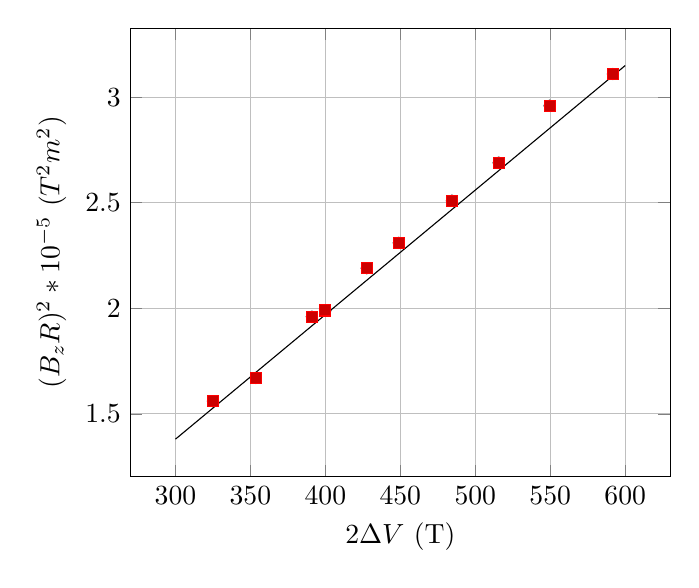
\begin{tikzpicture}
        \begin{axis}
        [
            xlabel={$2\Delta V$ (T)},
            ylabel={$(B_zR)^2*10^{-5}$ ($T^2m^2$)},
            grid=both,
            scatter/classes={
                a={mark=o,draw=black},
                b={mark=o,draw=black,fill=black}
            }
        ]
        \addplot[scatter,only marks,scatter src=explicit symbolic] 
            table[meta=label] {
              x     y    xerror yerror    label
            325     1.56   0.1     0.022      b
            353.6	1.67   0.1     0.014      a
            391	    1.96   0.1     0.014      a
            427.6	2.19   0.1     0.014      a
            449     2.31   0.1     0.014      a
            484.4   2.51   0.1       0        a
            515.6   2.69   0.1       0        a  
            549.6   2.96   0.1       0        a
            591.8   3.11   0.1       0        a
            400     1.99   0.1       0        a
         
        };
        \addplot+[
            only marks,
            error bars/.cd,
            x dir=both, x explicit,
            y dir=both, y explicit
        ] table[x=x, y=y, x error=xerror, y error=yerror] {
                x     y    xerror yerror    label
            325     1.56   0.1     0.022      b
            353.6	1.67   0.1     0.014      a
            391	    1.96   0.1     0.014      a
            427.6	2.19   0.1     0.014      a
            449     2.31   0.1     0.014      a
            484.4   2.51   0.1       0        a
            515.6   2.69   0.1       0        a  
            549.6   2.96   0.1       0        a
            591.8   3.11   0.1       0        a
            400     1.99   0.1       0        a
        };
        \addplot[
    domain=300:600,
    samples=100,
    color=black
] {0.0059*x - 0.39};
    \end{axis}
    \end{tikzpicture}
    \caption{Linear regression between $(B_zR)^2$ and the voltage for the orthogonal setup. }
\end{figure}

%paralello
\begin{figure}[H]
    \centering
    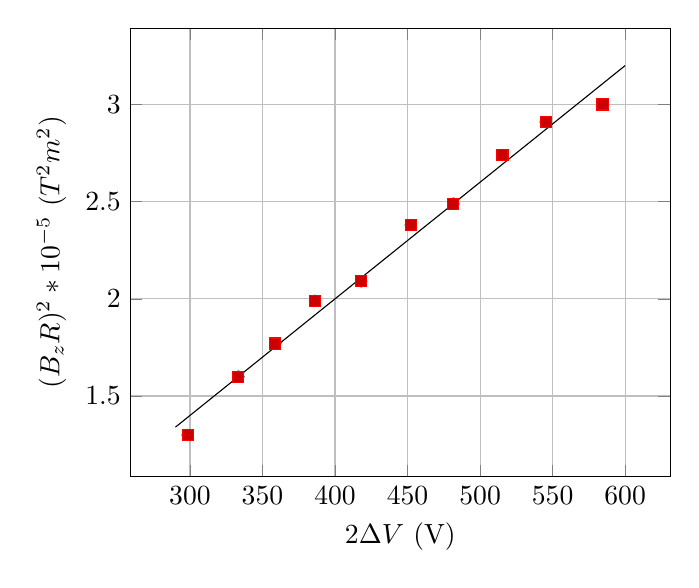
\begin{tikzpicture}
        \begin{axis}
        [
            xlabel={$2\Delta V$ (V)},
            ylabel={$(B_zR)^2*10^{-5}$ ($T^2m^2$)},
            grid=both,
            scatter/classes={
                a={mark=o,draw=black},
                b={mark=o,draw=black,fill=black}
            }
        ]
        \addplot[scatter,only marks,scatter src=explicit symbolic] 
            table[meta=label] {
              x     y    xerror yerror    label
            298.4   1.30   0.1     0.022      b
            333.4	1.60   0.1     0.014      a
            358.8   1.77   0.1     0.014      a
            386.2	1.99   0.1     0.014      a
            418     2.09   0.1     0.014      a
            452.2   2.38   0.1       0        a
            481.6   2.49   0.1       0        a  
            515.4   2.74   0.1       0        a
            545.2   2.91   0.1       0        a
            584.4   3.00   0.1       0        a
         
        };
        \addplot+[
            only marks,
            error bars/.cd,
            x dir=both, x explicit,
            y dir=both, y explicit
        ] table[x=x, y=y, x error=xerror, y error=yerror] {
             x     y    xerror yerror    label
            298.4   1.30   0.1     0.022      b
            333.4	1.60   0.1     0.014      a
            358.8   1.77   0.1     0.014      a
            386.2	1.99   0.1     0.014      a
            418     2.09   0.1     0.014      a
            452.2   2.38   0.1       0        a
            481.6   2.49   0.1       0        a  
            515.4   2.74   0.1       0        a
            545.2   2.91   0.1       0        a
            584.4   3.00   0.1       0        a
        };
        \addplot[
    domain=290:600,
    samples=100,
    color=black
] {0.0060*x - 0.40};
    \end{axis}
    \end{tikzpicture}
    \caption{Linear regression between $(B_zR)^2$ and the voltage for the parallel setup. }
\end{figure}

%antiparallelo

\begin{figure}[H]
    \centering
    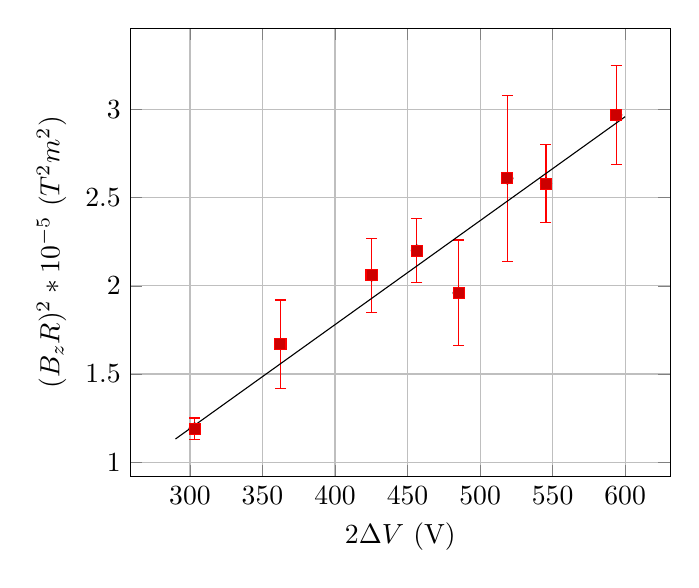
\begin{tikzpicture}
        \begin{axis}
        [
            xlabel={$2\Delta V$ (V)},
            ylabel={$(B_zR)^2*10^{-5}$ ($T^2m^2$)},
            grid=both,
            scatter/classes={
                a={mark=o,draw=black},
                b={mark=o,draw=black,fill=black}
            }
        ]
        \addplot[scatter,only marks,scatter src=explicit symbolic] 
            table[meta=label] {
              x     y    xerror yerror    label
            303.2   1.19   0.1     0.022      b
            362.4	1.67   0.1     0.014      a
            425.2   2.06   0.1     0.014      a
            485.2	1.96   0.1     0.014      a
            545.4   2.58   0.1     0.014      a
            593.8   2.97   0.1       0        a
            518.8   2.61   0.1       0        a  
            456.4   2.20   0.1       0        a
        };
        \addplot+[
            only marks,
            error bars/.cd,
            x dir=both, x explicit,
            y dir=both, y explicit
        ] table[x=x, y=y, x error=xerror, y error=yerror] {
               x     y    xerror yerror    label
            303.2   1.19   0.1     0.06      b
            362.4	1.67   0.1     0.25      a
            425.2   2.06   0.1     0.21      a
            485.2	1.96   0.1     0.30      a
            545.4   2.58   0.1     0.22      a
            593.8   2.97   0.1     0.28      a
            518.8   2.61   0.1     0.47      a  
            456.4   2.20   0.1     0.18      a
        };
        \addplot[
    domain=290:600,
    samples=100,
    color=black
] {0.0059*x - 0.58};
    \end{axis}
    \end{tikzpicture}
    \caption{Linear regression between $(B_zR)^2$ and the voltage for the antiparallel setup.}
\end{figure}
We can notice that the measure for the antiparallel setup are way more inaccurate, this has led to a higher uncertainty on respective the e/m value.
The reduced chi squared for each configuration are:
\begin{align*}
    &\chi_{red}^2=10.5\,\,(Orthogonal)\\
    &\chi_{red}^2=55.7\,\,(Parallel)\\
    &\chi_{red}^2=0.32\,\,(Antiparallel)
\end{align*}
the reduced chi squared for the orthogonal and parallel setup are completely out of scale, this would mean that our measure are utterly flawed. As we discussed later in the conclusion we thinks that this problem derive for an underestimation of the uncertainty on the beam radius.
The final values were found to be:
\begin{align*}
    &\frac{e}{m}=(1.69\pm0.01)\, \mathrm{C/Kg}\,\, (Orthogonal)\\
    &\frac{e}{m}=(1.66\pm0.01)\, \mathrm{C/Kg}\,\, (Parallel)\\
    &\frac{e}{m}=(1.67\pm0.16)\, \mathrm{C/Kg}\,\, (Antiparallel)\\
\end{align*}
two of them doesn't correlates with the accepted value of:
\begin{equation*}
    \frac{e}{m}=1.76\,\,\, \mathrm{C/Kg}
\end{equation*}



\subsection{Horizontal component's intensity of Earth's magnetic field}
For each fixed angle $\theta$ we measured the intensity I two times (clockwise $I_c$ and counter-clockwise $I_{cc}$) and took their mean as the final value:
\begin{table}[H]
\centering
\begin{tabular}{|c|c|c|c|c|}
\hline
$I_c$ (mA) & $I_{cc}$ (mA) & Mean I (mA) & $\theta$ \\ \hline
14.33 & 15.76 & 15.05 & 45  \\ \hline
17.30 & 20.20 & 18.75 & 50  \\ \hline
21.38 & 22.60 & 21.99 & 55  \\ \hline
26.55 & 26.29 & 26.42 & 60  \\ \hline
34.98 & 33.65 & 34.32 & 65  \\ \hline
\end{tabular}
\end{table}
The uncertainty on the intensity is the last digit provide by the device ($\pm 0.01$ mA) while the one on the angle is the protractor's resolution ($\pm 1^{\circ}$).
The coil magnetic field's components are tabulated for fixed $\theta$ and needle lenght R:
\begin{table}[H]
\centering
\begin{tabular}{|c|c|}
\hline
$B_z$ (mT) & $B_r$ (mT)\\ \hline
0.15438 & 0.00228 \\ \hline
0.15471 & 0.00167 \\ \hline
0.15480 & 0.00110 \\ \hline
0.15472 & 0.00062 \\ \hline
0.15450 & 0.00025 \\ \hline
\end{tabular}
\caption{Tabulated values for the orthogonal ($B_z$) and parallel ($B_r$) coil magnetic field's components.}
\end{table}

We can now calculate the Horizontal component of Earth's magnetic fiels ($B_t$) as:
\begin{equation*}
    B_t=\frac{I}{I_0}(B_z \cot{(\theta)}+B_r)
\end{equation*}
where $I_0=(100\pm 1)$ mA is the intensity of the coil current power source, and calculated its uncertainty:
\begin{align*}
    &\sigma_{B_t}^2 = \left( \frac{1}{I_0} \left( B_z \cot(\theta) + B_r \right) \sigma_I \right)^2 + \left( -\frac{I}{I_0^2} \left( B_z \cot(\theta) + B_r \right) \sigma_{I_0} \right)^2 + \left( \frac{I}{I_0} \cot(\theta) \sigma_{B_z} \right)^2 \\
    &+ \left( \frac{I}{I_0} B_z \left( -\csc^2(\theta) \right) \sigma_\theta \right)^2 + \left( \frac{I}{I_0} \sigma_{B_r} \right)^2
\end{align*}
Its values for each measurement are shown below:
\begin{table}[H]
\centering
\begin{tabular}{|c|c|}
\hline
$B_t$ ($\mu$T) & $\sigma_{B_z}$ ($\mu$T) \\
\hline
23.57 & 1.40 \\
\hline
24.65 & 2.11 \\
\hline
24.08 & 1.13 \\
\hline
23.76 & 0.99 \\
\hline
24.81 & 1.25 \\
\hline
\end{tabular}
\end{table}
We lastly calculated the final value as the weighted arithmetic mean of these values finding:
\begin{equation*}
    B_{tf}=(24.08\pm0.56)\,\, \mu\mathrm{T}
\end{equation*}

